\let\lesson\undefined
\newcommand{\lesson}{\phantomlesson{Bài 4: Chuyển động thẳng}}
\chapter[Vận tốc và đồ thị độ dịch chuyển - thời gian]{Vận tốc và đồ thị độ dịch chuyển - thời gian}
\setcounter{section}{0}
\section{Lý thuyết}
\subsection{Vận tốc}
\subsubsection{Vận tốc trung bình}
Vận tốc trung bình là đại lượng vectơ được xác định bằng thương số giữa độ dịch chuyển của vật và thời gian để vật thực hiện độ dịch chuyển đó
$$\overrightarrow{v_\text{tb}}=\dfrac{\vec{d}}{\Delta t}=\dfrac{\Delta \vec{x}}{\Delta t}$$
\luuy{Tốc độ trung bình chỉ bằng độ lớn của vận tốc trung bình khi vật chuyển động thẳng không đổi chiều.}
\subsection{Phương trình chuyển động thẳng đều}
Xét một chất điểm chuyển động thẳng đều trên đường thẳng O$x$ với tốc độ $v$. Ở thời điểm ban đầu ($t_0=0$), vật ở vị trí A cách gốc O một đoạn $x_0$. Vào thời điểm $t$, vật ở vị trí M cách gốc O một đoạn $x$.  
\begin{center}
\begin{tikzpicture}
	\coordinate (O) at (0,0);
	\coordinate (A) at (2,0);
	\coordinate (M) at (5,0);
	\coordinate (x) at (8,0);
	\coordinate (O1) at ($(O)-(0,1cm)$);
	\coordinate (A1) at ($(A)-(0,1cm)$);
	\draw[->,thick] (O) -- (x);
	\foreach \i in {O,A}{
		\filldraw[black] (\i) circle (0.5mm);
	}
	\node[label=90:O] at (O){};	
	\node[label=90:A] at (A){};
	\node[label=90:M] at (M){};	
	\node[label=90:x] at (x){};	
	\draw[<->] (O1) -- (A1);
	\node [fill=white] (F1) at ($(O1)!0.5!(A1)$) {$x_0$};
	\coordinate (M1) at ($(M)-(0,1cm)$);
	\draw[<->] (A1) -- (M1);
	\node [fill=white] (F2) at ($(A1)!0.5!(M1)$) {$s$};
	\coordinate (O2) at ($(O)-(0,1.5cm)$);
	\coordinate (M2) at ($(M)-(0,1.5cm)$);
	\draw[<->] (O2) -- (M2);
	\node [fill=white] (F3) at ($(O2)!0.5!(M2)$) {$x$};
	\draw[dashed] (O) -- (O2);
	\draw[dashed] (A) -- (A1);
	\draw[dashed] (M) -- (M2);
	\filldraw[blue] (M) circle (0.5mm);
	%		\node[above of=O]()
\end{tikzpicture}
\end{center}

Tọa độ của chất điểm sau thời gian chuyển động $t$ là:
\begin{equation}
x=x_0+s=x_0+vt.
\end{equation}
Phương trình dùng để xác định tọa độ của M theo thời gian được gọi là phương trình chuyển động của chất điểm M. Trong trường hợp này, M chuyển động thẳng đều nên phương trình này gọi là phương trình chuyển động thẳng đều của điểm M. 
\subsection{Đồ thị độ dịch chuyển - thời gian}
Đồ thị độ dịch chuyển - thời gian của hai vật A và B được mô tả như hình \ref{fig:5.1}
\begin{center}
	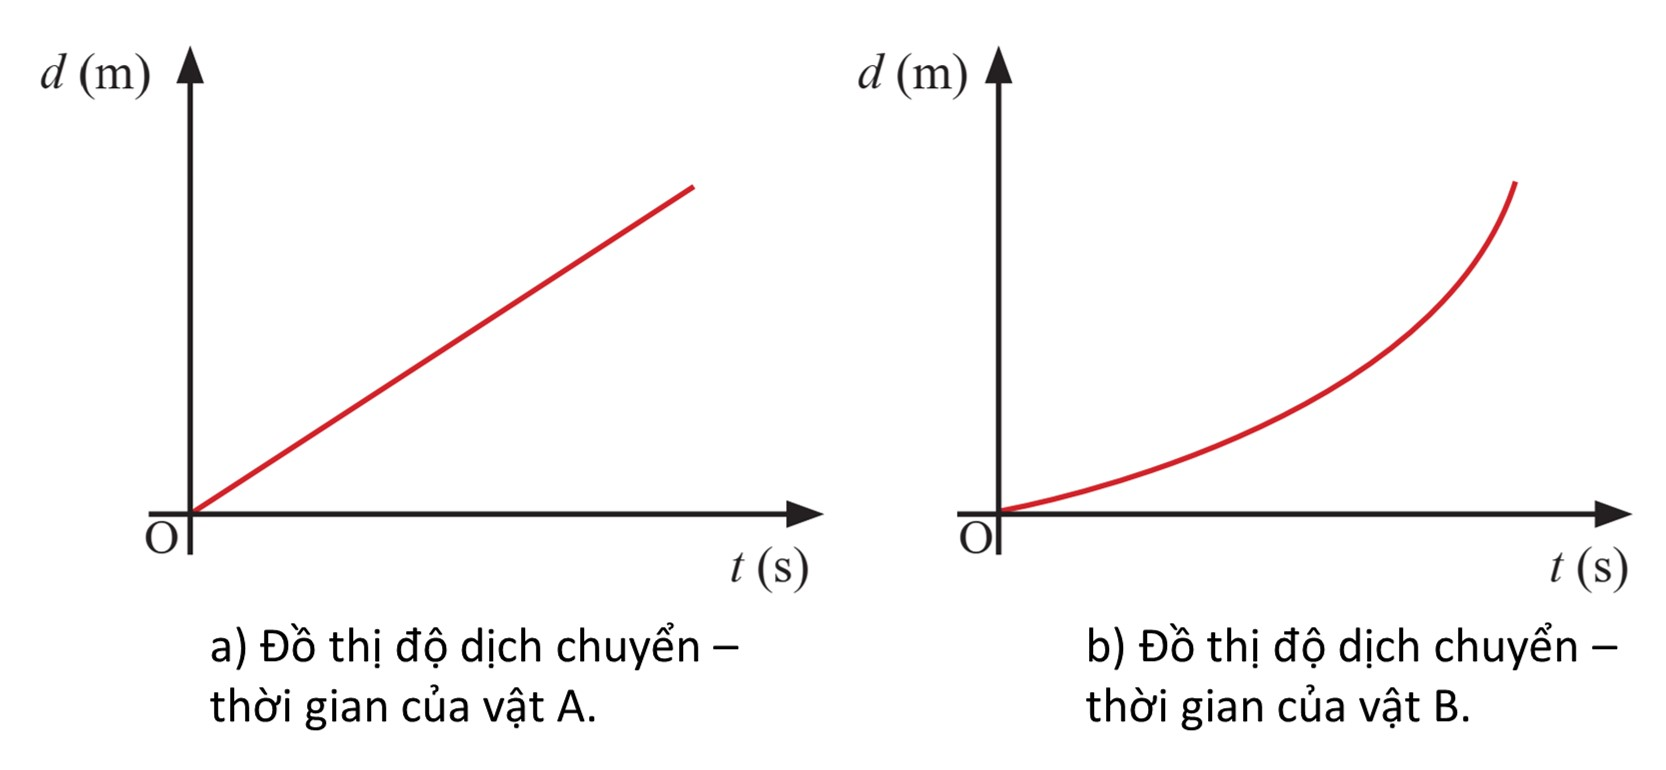
\includegraphics[width=0.6\linewidth]{../figs/VN10-2023-PH-TP005-1}
	\captionof{figure}{}
	\label{fig:5.1}
\end{center}
Từ các đồ thị $\left(d-t\right)$, ta có nhận xét:
\begin{enumerate}[label=\alph*)]
	\item Đồ thị $\left(d-t\right)$ mô tả chuyển động của vật $A$ là đường thẳng đi qua gốc toạ độ. Chuyển động của vật $A$ là chuyển động thẳng đều.
	\item Đồ thị $\left(d-t\right)$ mô tả chuyển động của vật $B$ là đường cong qua gốc toạ độ. Độ dịch chuyển của vật B trong những khoảng thời gian bằng nhau tăng lên nên chuyển động của vật B là chuyển động thẳng nhanh dần.
\end{enumerate}
\subsubsection{Xác định vận tốc từ độ dốc của đồ thị $\left(d-t\right)$}
\textbf{Xác định vận tốc trung bình từ đồ thị độ dịch chuyển - thời gian}\\
Xét vật chuyển động từ vị trí 1 (tại thời điểm $t_1$) đến vị trí 2 (tại thời điểm $t_2$) lần lượt được biểu diễn bởi hai điểm $P$ và $Q$ trên đồ thị ($d$ – $t$) trong hình \ref{fig:5.2}. So sánh với biểu thức để xác định vận tốc trung bình, ta có: độ dịch chuyển $d$ của vật chính là đoạn $HQ$, khoảng thời gian $\Delta t$ chính là độ dài $PH$.\\
\begin{center}
	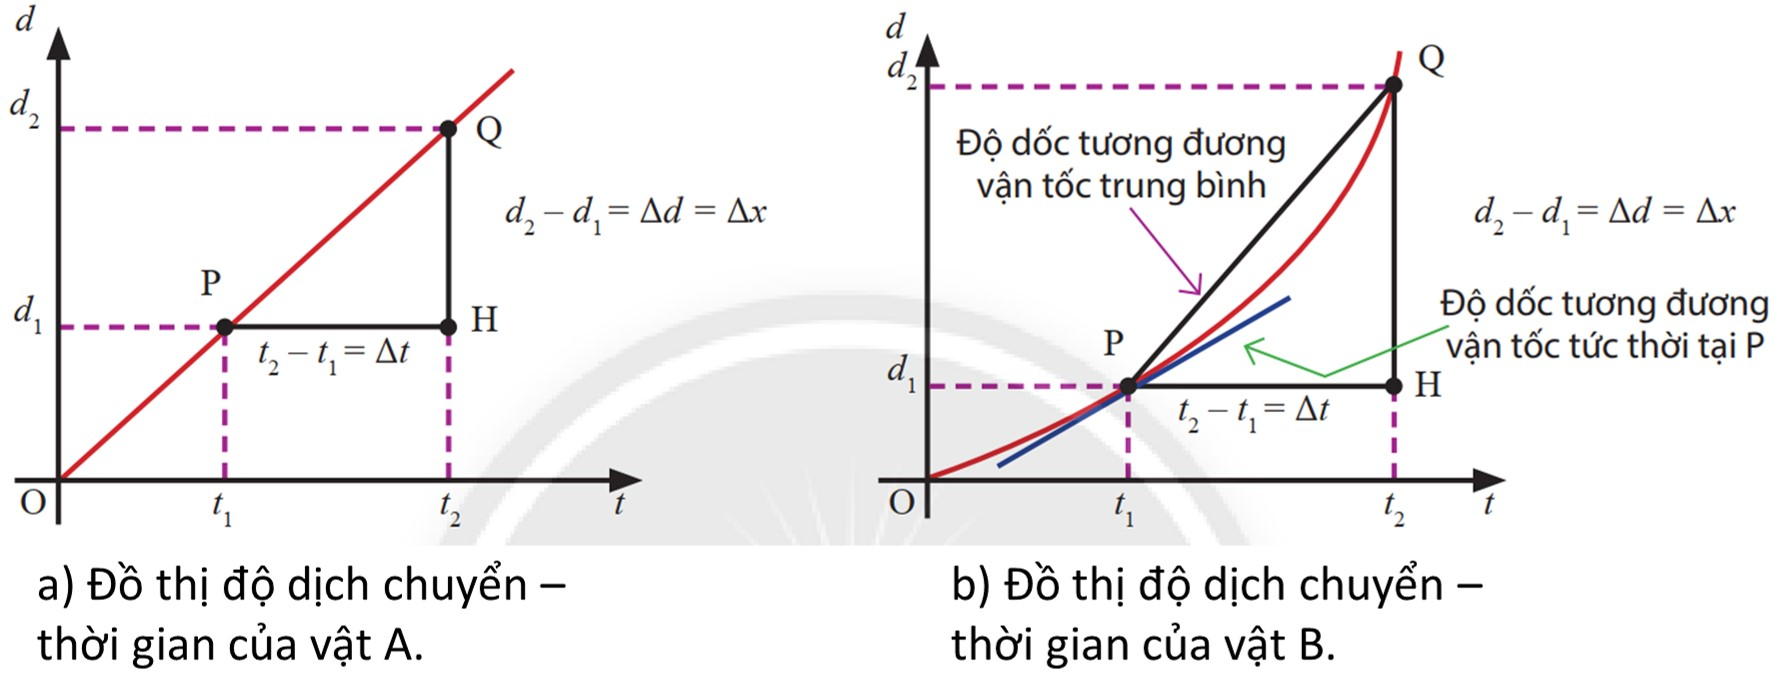
\includegraphics[width=0.8\linewidth]{../figs/VN10-2023-PH-TP005-2}
	\captionof{figure}{}
	\label{fig:5.2}
\end{center}
Từ đó, ta thấy vận tốc trung bình chính là độ dốc của đoạn $PQ$ nối hai điểm trên đồ thị biểu diễn vị trí đầu đến vị trí cuối của vật.\\
\textbf{Xác định vận tốc tức thời từ đồ thị độ dịch chuyển - thời gian}\\
Vận tốc tức thời của vật tại một thời điểm được xác định bởi độ dốc của tiếp tuyến với đồ thị ($d$ - $t$) tại thời điểm đang xét.\\
Tốc độ tức thời tại một thời điểm chính là độ lớn của độ dốc tiếp tuyến của đồ thị ($d$ - $t$) tại điểm đó.
\section{Mục tiêu bài học - Ví dụ minh họa}
\begin{dang}{Nhận biết được phương trình chuyển động thẳng đều}
	\viduii{2}{ Trong các phương trình chuyển động thẳng đều sau đây, phương trình nào biểu diễn chuyển động không xuất phát từ gốc tọa độ và ban đầu hướng về gốc tọa độ:
		\begin{mcq}(2)
			\item $x = 80 - 30t.$
			\item $x = 15 + 40t.$
			\item $x = -6t.$
			\item $x = -10 - 6t.$
		\end{mcq}
	}
	{\hide{
		Phương trình chuyển động của vật là 
		$$x=x_0 +vt.$$	
		Chuyển động không xuất phát từ gốc tọa độ thì $x_0 \neq  0$.
		
		Ban đầu vật hướng về gốc tọa độ thì vị trí ban đầu và vận tốc của vật phải thỏa mãn 
		\begin{equation*}
			\left\lbrace
			\begin{array}{rl}
				x_0&<0,\\
				v&>0
			\end{array}
			\right.
			\qquad\text{hoặc}\qquad
			\left\lbrace
			\begin{array}{rl}
				x_0&>0,\\
				v&<0
			\end{array}
			\right.
		\end{equation*}
		Hình vẽ sau minh họa hai trường hợp này.
		\begin{center}
			\begin{tikzpicture}
				\coordinate (O) at (0,0);
				\coordinate (A) at (-3,0);
				\coordinate (A1) at ($(A)+(1,0)$);
				\coordinate (M) at (4,0);
				\coordinate (M1) at ($(M)-(1,0)$);
				\coordinate (x) at (6,0);
				\coordinate (X) at (-4,0);
				\draw[->] (X) -- (x);
				\foreach \i in {O,A,M}{
					\filldraw[black] (\i) circle (0.5mm);
				}
				\draw[->,very thick,blue] (A) -- (A1);
				\draw[->,very thick,red] (M) -- (M1);
				\node[label=90:O] at (O){};	
				\node[label=90:$\vec{v}$]at (A1){};
				\node[label=90:$\vec{v}$]at (M1){};
				\node[align=center,below=0.2cm of A](Mnode){$x_0<0$\\$v>0$};
				\node[align=center,below=0.2cm of M](Mnode){$x_0>0$\\$v<0$};
				\node[label=90:$x$]at (x){};
			\end{tikzpicture}
		\end{center}
		Trong các lựa chọn, chỉ có lựa chọn A ($x = 80 - 30t$) thỏa mãn với điều kiện trên.
		
		\textbf{Đáp án: A}.
	}}
\end{dang}

\begin{dang}{Xây dựng phương trình, tính các đại lượng\\ trong phương trình chuyển động thẳng đều\\ cho một hoặc hai vật.}
	\viduii{2}{Một vật chuyển động thẳng đều với tốc độ $\SI{2}{m/s}$. Lúc $t = \SI{2}{s}$ vật có tọa độ $\SI{5}{m}$. Phương trình chuyển động của vật là 
		\begin{mcq}(2)
			\item $x=2t+1\qquad\left(\si{\meter}, \si{\second}\right)$.
			\item $x=-2t +5\qquad\left(\si{\meter}, \si{\second}\right)$.
			\item $x=2t+5\qquad\left(\si{\meter}, \si{\second}\right)$.
			\item $x=-2t+1\qquad\left(\si{\meter}, \si{\second}\right)$.
		\end{mcq}
	}
	{\hide{
		Phương trình tọa độ của vật có dạng: 
		$$x=x_0 +vt.$$
		
		Thay $x=\SI{5}{m}$, $v=\SI{2}{m/s}$, $t=\SI{2}{s}$ vào ta suy ra 
		\begin{align*}
			x_0=x-vt=\SI{5}{m}-\SI{2}{\meter/\second}\cdot\SI{2}{s}=\SI{1}{m}.
		\end{align*}
		
		Vậy phương trình chuyển động của vật là:
		
		$$x=1+2t =2t+1\qquad\left(\si{\meter}, \si{\second}\right).$$
		
		\textbf{Đáp án: A}.
	}}

	\viduii{3}{	Trên đường thẳng từ nhà đến chỗ làm việc của A, cùng một lúc xe 1 khởi hành từ nhà đến chỗ làm với $v_1=\SI{80}{\km/\hour}$. Xe 2 từ chỗ làm đi cùng chiều xe 1 với $v_2=\SI{60}{\km/\hour}$. Biết quãng đường từ nhà đến chỗ làm là $\SI{40}{\km}$. Lập phương trình chuyển động của mỗi xe với cùng hệ quy chiếu.
	}
	{\hide{
		Chọn hệ quy chiếu gồm:
		\begin{itemize}
			\item Chiều dương cùng chiều với chiều chuyển động với hai xe;
			\item Gốc tọa độ tại A;
			\item Mốc thời gian lúc hai xe bắt đầu xuất phát.
		\end{itemize}
		
		Xe 1 có phương trình chuyển động
		\begin{equation*}
			x_1=x_0 + v_1t = 80t\textrm{ (km, h)}.
		\end{equation*}
		Xe 2 có phương trình chuyển động  
		\begin{equation*}
			x_2=x_0 + v_2t = 40+60t\textrm{ (km, h)}.
		\end{equation*}
	}}


	\viduii{3}{	Hai vật chuyển động ngược chiều qua A và B cùng một lúc. Vật qua A có tốc độ $v_1=\SI{10}{\meter/\second}$, vật qua B có tốc độ $v_2=\SI{15}{\meter/\second}$. Cho biết AB có chiều dài $\SI{100}{m}$. Lấy trục tọa độ là đường thẳng AB, gốc tọa độ ở B, chiều dương từ A sang B, mốc thời gian là lúc chúng cùng qua A và B. Lập phương trình chuyển động của mỗi vật.
	}
	{\hide{
		Hệ quy chiếu gồm:
		\begin{itemize}
			\item Gốc tọa độ tại B;
			\item Chiều dương từ A sang B;
			\item Mốc thời gian lúc hai vật cùng qua A và B.
		\end{itemize}
		
		Phương trình chuyển động của vật qua A là
		\begin{equation*}
			x_\text{A}=x_{0\text{A}} + v_\text{A}t =-100+10t\textrm{ (m, s)}.
		\end{equation*}
		
		Phương trình chuyển động của vật qua B là
		\begin{equation*}
			x_\text{B}=x_{0\text{B}} + v_\text{B}t = -15t\textrm{ (m, s)}.
		\end{equation*}
		
	}}
\end{dang}

\begin{dang}{Xác định vị trí, thời điểm \\hai vật chuyển động thẳng đều gặp nhau}
\viduii{3}{	Hai vật chuyển động ngược chiều qua A và B cùng một lúc. Vật qua A có tốc độ $v_1=\SI{10}{\meter/\second}$, vật qua B có tốc độ $v_2=\SI{15}{\meter/\second}$. Cho biết AB có chiều dài $\SI{100}{m}$. Xác định vị trí và thời điểm chúng gặp nhau.
	
}
{\hide{
	Chọn gốc tọa độ ở vị trí A, gốc thời gian ở thời điểm hai vật đang ở A và B. Chiều dương trục toạ độ hướng từ A sang B.\\
	Phương trình chuyển động của hai vật:
	\begin{equation*}
		\begin{cases}
			x_1=x_{01}+v_1t\\
			x_2=x_{02}+v_2t
		\end{cases}
	\Rightarrow
	\begin{cases}
		x_1=10t\\
		x_2=100-15t
	\end{cases}
\left(\si{\meter}, \si{\second}\right)
	\end{equation*}
	Hai vật gặp nhau khi chúng có cùng tọa độ
	\begin{equation*}
		x_\text{1}=x_\text{2}\Rightarrow 10t=100-15t \Rightarrow t=\SI{4}{\second}.
	\end{equation*}
	Dựa vào phương trình chuyển động, ta xác định được vị trí hai vật gặp nhau 
	\begin{equation*}
		x_\text{1}=x_\text{2}=10t=\SI{40}{\meter}.
	\end{equation*}
}}

\viduii{3}{Lúc 7 giờ, một người ở A chuyển động thẳng đều với tốc độ $ v_A= \SI{36}{km/h}$ đuổi theo người ở B đang chuyển động với tốc độ $v_B = \SI{5}{m/s}$. Biết $AB = \SI{18}{km}$. Hai người đuổi kịp nhau tại nơi cách A một khoảng 
	\begin{mcq}(4)
		\item $\SI{58}{km}$.
		\item $\SI{46}{km}$.
		\item $\SI{36}{km}$.
		\item $\SI{24}{km}$.
	\end{mcq}
}
{\hide{
	$v_B = \SI{5}{m/s}=\SI{18}{\kilo\meter/\hour}$\\
	Chọn gốc toạ độ tại A, chiều dương trục toạ độ hướng từ A đến B, gốc thời gian lúc 7 giờ.\\
	Phương trình chuyển động của hai người ở A và B:
	\begin{equation*}
		\begin{cases}
			x_\text{A}=36t\\
			x_\text{B}=18+18t
		\end{cases}
	\left(\si{\meter}, \si{\second}\right)
	\end{equation*}
	Khi hai người gặp nhau, tọa độ của hai người trùng nhau  
	\begin{align*}
		x_1&=x_2 \quad
		\Rightarrow\quad 36t=18+18t\quad\Rightarrow\quad t=\SI{1}{h}
	\end{align*}
	Dựa vào phương trình chuyển động, suy ra nơi gặp nhau cách A
	$$x_\text{A}  =36t=\SI{36}{\kilo\meter/\hour}\cdot\SI{1}{\hour}= \SI{36}{km}.$$
	
	
	\textbf{Đáp án: C}.
}}
\end{dang}

\begin{dang}{Thực hiện xác định quãng đường, vận tốc và thời gian dựa vào phương trình chuyển động thẳng đều}
	\viduii{3}{Xe thứ nhất đi từ A đến B mất 8 giờ, xe thứ hai đi từ B đến A mất 6 giờ. Nếu hai xe khởi hành cùng một lúc từ A và B để đến gần nhau thì sau 3 giờ hai xe cách nhau $\SI{30}{km}$. Tính chiều dài của quãng đường AB.
	}
	{\hide{
		Gọi $v_1$; $v_2$ lần lượt là tốc độ của xe thứ nhất và xe thứ hai. Từ quãng đường AB và thời gian chuyển động, ta tính được tỉ số tốc độ của hai xe
		\begin{align*}
			v_1&=\dfrac{s}{t_1},\\
			v_2&=\dfrac{s}{t_2},\\
			\Rightarrow \dfrac{v_1}{v_2}&=\dfrac{t_2}{t_1}=\dfrac{\SI{6}{\hour}}{\SI{8}{\hour}}=\dfrac{3}{4}\\
			\Rightarrow v_1&=\dfrac{3}{4} v_2.
		\end{align*}
		
		Nếu chọn gốc tọa độ tại vị trí A, chiều dương từ A đến B và gốc thời gian là lúc 2 xe xuất phát thì phương trình chuyển động của mỗi xe:
		\begin{align*}
			x_1 &=v_1t=\dfrac{3}{4}v_2 t,\\
			x_2&=s-v_2t=v_2t_2-v_2t.
		\end{align*}
		
		Sau 3 giờ: $$|x_1-x_2|=\SI{30}{km} \Rightarrow v_2=\SI{40}{km/h}.$$
		
		Chiều dài của quãng đường AB: $$s=v_2t_2=\SI{40}{\kilo\meter/\hour}\cdot\SI{6}{\hour} =\SI{240}{km}.$$
		
	}}
	
\viduii{3}{Hai vật chuyển động ngược chiều qua A và B cùng một lúc. Vật qua A có tốc độ $v_1=\SI{10}{\meter/\second}$, vật qua B có tốc độ $v_2=\SI{15}{\meter/\second}$. Cho biết AB có chiều dài $\SI{100}{m}$. Xác định vị trí và thời điểm chúng cách nhau $\SI{25}{\meter}$.
}
{\hide{
	Chọn gốc tọa độ ở A, chiều dương trục toạ độ hướng từ A đến B và gốc thời gian là thời điểm hai vật đang đi qua A và B. Gọi $s=\SI{100}{\meter}$ là chiều dài đoạn AB. Phương trình chuyển động của hai vật lần lượt là 
	\begin{equation}
		\begin{cases}
			x_1&=v_1t\\
			x_2&=s-v_2t
		\end{cases}
	\Rightarrow \begin{cases}
		x_1=10t\\
		x_2=100-15t
	\end{cases}
\left(\si{\meter}, \si{\second}\right)
	\end{equation}	
	Khi hai vật cách nhau $d=\SI{25}{\meter}$
	\begin{equation*}
		d=\left|x_\text{A}-x_\text{B}\right|=\SI{25}{\meter}.
	\end{equation*}
	\begin{align*}
	\Leftrightarrow	\left|10t-100+15t\right|=25\Rightarrow t=\SI{3}{\second} \vee t=\SI{5}{\second}.
	\end{align*}
\begin{itemize}
	\item 	Với $t=\SI{3}{\second}$, thay vào phương trình chuyển động, ta được vị trí hai vật
	\begin{align*}
		\begin{cases}
			x_\text{1}=v_1t=\left(\SI{10}{\meter/\second}\right)\cdot\left(\SI{3}{\second}\right)=\SI{30}{\meter}\\
			x_\text{2}=s-v_2t=\SI{100}{\meter}-\left(\SI{15}{\meter/\second}\right)\cdot\left(\SI{3}{\second}\right)=\SI{55}{\meter}.
		\end{cases}
	\end{align*}
\item Với $t=\SI{5}{\second}$, thay vào phương trình chuyển động, ta được vị trí hai vật 
\begin{align*}
	\begin{cases}
		x_\text{1}=v_1t=\left(\SI{10}{\meter/\second}\right)\cdot\left(\SI{5}{\second}\right)=\SI{50}{\meter}\\
		x_\text{2}=s-v_2t=\SI{100}{\meter}-\left(\SI{15}{\meter/\second}\right)\cdot\left(\SI{5}{\second}\right)=\SI{25}{\meter}.
	\end{cases}
\end{align*}
\end{itemize}
}}

\end{dang}
\begin{dang}{Tính được tốc độ từ độ dốc của đồ thị độ dịch chuyển – thời gian.}
	\viduii{2}
	{Một vật chuyển động có đồ thị ($d$-$t$) được mô tả như hình \ref{fig:5.3}. Hãy xác định tốc độ tức thời của vật tại các vị trí $A, B$ và $C$.
		\begin{center}
			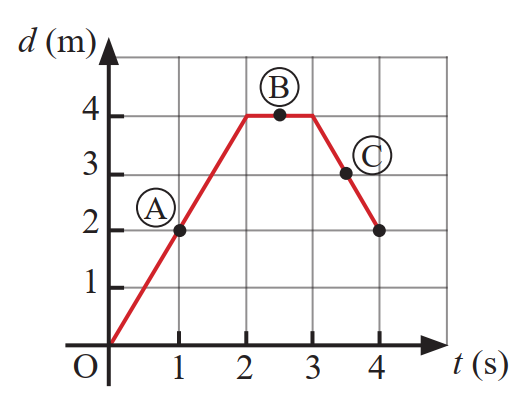
\includegraphics[width=0.35\linewidth]{../figs/VN10-2023-PH-TP005-3}
			\captionof{figure}{}
			\label{fig:5.3}
		\end{center}
	}
	{\hide{
		Tốc độ tức thời tại một thời điểm chính là độ dốc của tiếp tuyến với đồ thị ($d$ - $t$) tại điểm đó:
	\begin{itemize}
		\item Tốc độ tức thời tại $A$
		$$v_A=\dfrac{\left|2-0\right|}{1-0}=\SI{2}{\meter/\second}$$
		\item Tốc độ tức thời tại điểm $B$
		$$v_B=\dfrac{\left|4-4\right|}{3-2}=\SI{0}{\meter/\second}$$
		\item Tốc độ tức thời tại điểm $C$
		$$v_C=\dfrac{\left|2-4\right|}{4-3}=\SI{2}{\meter/\second}$$
	\end{itemize}
	}}

\viduii{3}
{Đồ thị độ dịch chuyển – thời gian trong chuyển động thẳng của một xe ô tô đồ chơi điều khiển từ xa được vẽ ở hình \ref{fig:5.4}.
	\begin{center}
		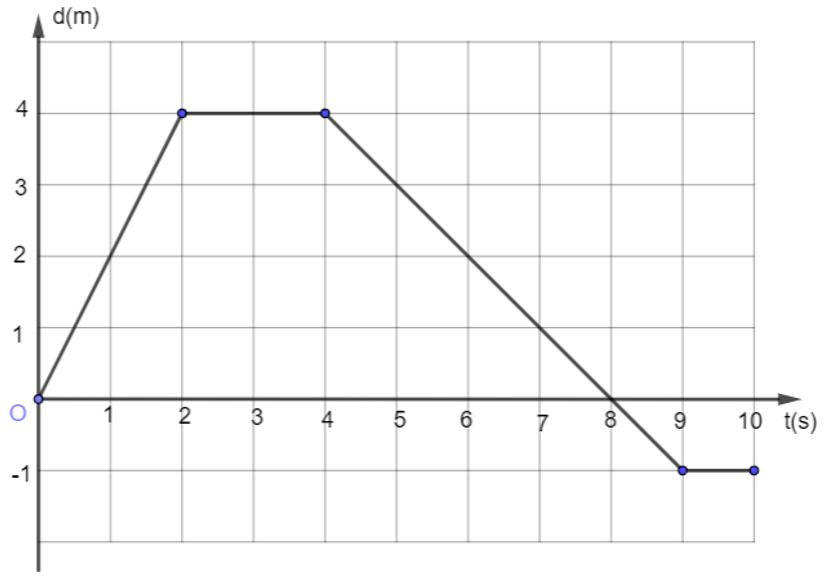
\includegraphics[width=0.5\linewidth]{../figs/VN10-2023-PH-TP005-4}
		\captionof{figure}{}
		\label{fig:5.4}
	\end{center}
	\begin{enumerate}[label=\alph*)]
		\item Mô tả chuyển động của xe.
		\item Xác định vị trí của xe so với điểm xuất phát của xe ở giây thứ 2, giây thứ 4, giây thứ 8 và giây thứ 10.
		\item Xác định tốc độ và vận tốc của xe trong 2 giây đầu, từ giây 2 đến giây 4 và từ giây 4 đến giây 8.
		\item Xác định quãng đường đi được và độ dịch chuyển của xe sau 10 giây chuyển động. Tại sao giá trị của chúng không giống nhau?
	\end{enumerate}
	
}
{\hide{
\begin{enumerate}[label=\alph*)]
	\item \begin{itemize}
		\item Trong 2 giây đầu xe chuyển động với vận tốc không đổi.
		\item Từ giây 2 đến giây 4 xe dừng lại.
		\item Từ giây 4 đến giây 8 xe đổi chiều chuyển động theo hướng ngược lại với vận tốc nhỏ hơn lúc đi và quay lại vị trí xuất phát.
		\item Từ giây 8 đến giây 9 xe đi tiếp với vận tốc đó thêm 1 đoạn rồi mới dừng lại.
		\item Từ giây 9 đến giây 10 xe dừng lại.
	\end{itemize}
	\item \begin{itemize}
		\item Ở giây thứ 2: xe cách vị trí xuất phát $\SI{4}{\meter}$.
		\item Ở giây thứ 4: xe vẫn cách vị trí xuất phát $\SI{4}{\meter}$.
		\item Ở giây thứ 8: xe quay lại vị trí xuất phát.
		\item Ở giây thứ 10: xe ở sau vị trí xuất phát $\SI{1}{\meter}$.
	\end{itemize}
	\item \begin{itemize}
		\item Trong 2 giây đầu: vận tốc của xe = tốc độ của xe $=\dfrac{\left|4-0\right|}{2-1}=\SI{2}{\meter/\second}$.
		\item Từ giây 4 đến giây 8
		\begin{itemize}
			\item tốc độ của xe $=\dfrac{\left|0-4\right|}{8-4}=\SI{1}{\meter/\second}$.
			\item vận tốc của xe $=\dfrac{0-4}{8-4}=\SI{-1}{\meter/\second}$.
		\end{itemize}
	\end{itemize}
	\item Sau 10 giây chuyển động thì 
	\begin{itemize}
		\item quãng đường xe đi được là $s=4+0+4+1=\SI{9}{\meter}$.
		\item độ dịch chuyển: $d=\SI{-1}{\meter}$.
	\end{itemize}
	Khi vật chuyển động thẳng, có đổi chiều thì quãng đường đi được và độ dịch chuyển có độ lớn không bằng nhau.
\end{enumerate}
}}
\end{dang}
\begin{dang}{Xây dựng đồ thị tọa độ - thời gian,\\ chọn tỉ xích, lập bảng giá trị tương ứng \\cho một vật chuyển động thẳng đều}
	\viduii{2}{Vật chuyển động thẳng đều có đồ thị tọa độ - thời gian như hình vẽ. Phương trình chuyển động của vật có dạng nào sau đây?
		\begin{center}
			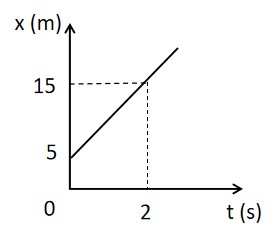
\includegraphics[scale=0.6]{../figs/VN10-PH-03-L-002-4-V2-01.jpg}
		\end{center}
		\begin{mcq}(4)
			\item $x=5+5t$.
			\item $x=4t$.
			\item $x=5-5t$.
			\item $x=5+4t$.
		\end{mcq}
	}
	{\hide{
		Nhận xét rằng đồ thị mô tả chuyển động của vật đi qua các điểm (\SI{0}{\second},\SI{5}{\meter}) và $(\SI{2}{\second},\SI{15}{\meter})$. Vận tốc của vật được tính từ tọa độ các điểm này 
		\begin{equation*}
			v=\dfrac{x-x_0}{t-t_0}=\dfrac{\SI{15}{\meter}-\SI{5}{\meter}}{\SI{2}{\second}-\SI{0}{\second}}=\SI{5}{\meter/\second}.
		\end{equation*}
		
		Phương trình chuyển động của vật do đó có dạng 
		\begin{equation*}
			x=x_0+vt=5+5t\textrm{ (m, s)}.
		\end{equation*}
		
		\textbf{Đáp án: A}.
	}}

	\viduii{3}{	Hai xe chuyển động đều trên cùng một đường thẳng, cùng chiều. Tốc độ của xe (I) là $\SI{20}{\meter/\second}$, tốc độ của xe (II) là $\SI{10}{\meter/\second}$. Lúc $t=0$, hai xe cách nhau $\SI{200}{\meter}$. Chọn gốc tọa độ là vị trí của xe (I) lúc $t=0$, chiều dương là chiều chuyển động của hai xe.
		\begin{enumerate}[label=\alph*)]
			\item Viết phương trình chuyển động của mỗi xe.
			\item Vẽ đồ thị chuyển động của hai xe, từ đồ thị hãy xác định thời điểm và nơi gặp nhau của hai xe.
		\end{enumerate}
	}
	{\hide{
		\begin{enumerate}[label=\alph*)]
			\item
			Hệ quy chiếu gồm:
			\begin{itemize}
				\item Gốc tọa độ là vị trí của xe (I) lúc $t=0$;
				\item Chiều dương là chiều chuyển động của hai xe;
				\item Mốc thời gian ($t=0$) là lúc hai xe cách nhau $\SI{200}{\meter}$.
			\end{itemize}
			
			Phương trình chuyển động của vật (I) là:
			\begin{equation*}
				x_\text{(I)}=x_{0\text{(I)}} + v_\text{(I)}t =20t\textrm{ (m, s)}.
			\end{equation*}
			
			Phương trình chuyển động của vật (II) là:
			\begin{equation*}
				x_\text{(II)}=x_{0\text{(II)}} + v_\text{(II)}t = 200+10t\textrm{ (m, s)}.
			\end{equation*}
			\item
			Đồ thị chuyển động của hai xe là:
			\begin{center}
				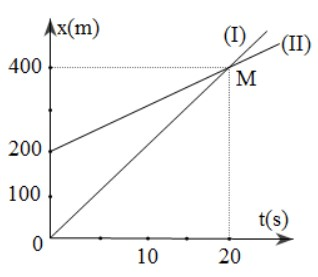
\includegraphics[scale=0.8]{../figs/VN10-PH-03-L-002-4-V2-02.jpg}
			\end{center}
			Hai đồ thị cắt nhau tại M ($t_M=\SI{20}{\second}$, $x_M=\SI{400}{\meter}$). Do đó, nơi gặp cách vị trí xe (I) lúc $t=0$ là $\SI{400}{\meter}$ sau thời gian $\SI{20}{\second}$.
		\end{enumerate}	
	}}
\end{dang}
